%!TEX root = main.tex
\chapter{Introduction}\label{chapter:introduction}
Mankind always have been pursued to find their location and position in world correctly. By advancement of science and using of new electronic devices, this requirement have been resolved. 

Generally for locating, we need a reference point as origin or (0,0,0) to express the location of an object in every moment relative to this reference. This procedure will be more complicated when the desired object is moving. To estimate the position of moving objects in each moment, the difference of displacement is calculated and updated.

Augmented Reality (AR) is a new technology that aims to generate a composite view for users. This view is a combination of the real view that user can see it and a virtual view such as graphics, sounds or animations which is generated by computer. To augment the additional information to the real world, the geometric relation between the world and the camera is necessary. These geometric relations that describes the position of the camera relative to reference point in every moment is called tracking.

Tracking an object is a fundamental part of Augmented Reality (AR). Tracking means finding the location of an object or camera when they have movement in a sequence of frames relative to a reference point. Based on the AR application and degree of freedom of the object and the camera, there are two main tracking approaches:

\begin{itemize}
\item 2D Tracking: Estimate a 2D transformation which describes the 3D displacement of the image projection of objects or parts of objects.
\item 3D Tracking: Identify the camera rotation and translation relative to the scene. It contains 6 degrees of freedom for rotation and translation. \autoref{fig:pnp_sampel} shows the rotation and translation between the camera and world coordinate. \footnote{\url{http://docs.opencv.org/trunk/doc/tutorials/calib3d/real_time_pose/real_time_pose.html}}.
\end{itemize}

\begin{figure}[H]
  \centering
  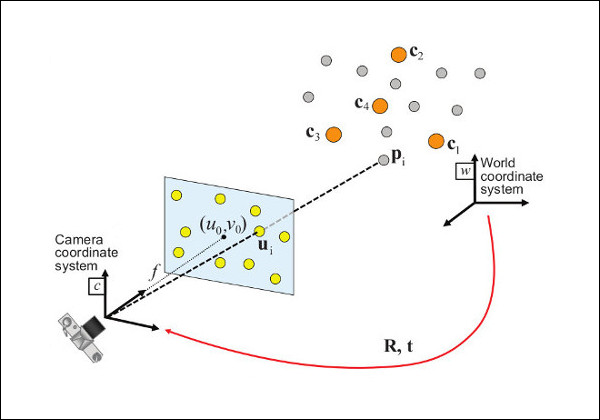
\includegraphics[width=140mm]{figures/pnp}
  \caption{3D Tracking: Finding the pose of camera relative to the world coordinate.} \label{fig:pnp_sample}
\end{figure}

Due to the diverse applications areas and existence of different mathematical approaches for solving the 3D tracking using a single camera, research in this field is substantially huge. Marker-based and Features-based techniques, are two methods to find out the position of camera or tracking of 3D objects.

\section{Motivation}
An accurate and robust estimation of camera pose is always a critical problem in some of computer vision applications. In augmented reality applications, two well-know techniques are used based on the knowledge that we have about the environment and type of applications: marker-based and feature-based approaches. 

This master thesis tries to implement a feature-based approach with using the state-of-the-art algorithms for all tasks that are necessary for estimating the pose of monocular camera. Improvement of accuracy and performance of camera pose estimation has been one of the motivations of this work. The existing open problems in case of feature matching also motivated the implementation of a robust feature matching and investigating its effect on the feature-based pose estimation. 

To evaluate the effectiveness of ours approach we implemented it inside the Ubitrack Framework (\autoref{sebsec:ubitrack}). There is already a marker-based approach in Ubitrack, but the framework lacks a feature-based implementation. In course of this master thesis we also implemented two robust feature matching and bundle adjustment modules for Ubitrack that have a positive effect on our result.

\section{Related Work}
\subsection{PTAM}
Georg Klein and David Murry \cite{klein2007parallel} proposed a method of estimating the pose (rotation and translation) of a camera without any prior knowledge about an small AR environment. The idea was adapted from Simultaneous Localization and Mapping (SLAM) algorithms in robotics with a novelty in implementation. Similar to both SLAM and Structure from Motion (SfM), the whole procedure can be divided into two major tasks:
\begin{itemize}
\item Mapping: create a set of 3D feature points from environment that are seen from camera. This 3D world is used to increase the accuracy of tracking task.
\item Tracking: estimating the pose of camera with using the 3D map that are produced in previous step. In this approach the camera pose are computed by two levels. Estimating the initial pose and then the precise pose.
\end{itemize}
The key difference of PTAM algorithm compared to the simple SLAM and SFM is the use of two parallel processing threads for executing the tracking and mapping tasks. This allows to do this operation in the real-time.

Likewise, after each mapping task, the obtained 3D points are optimized by a bundle adjustment that is called local bundle adjustment. Furthermore, after a long iteration, a global bundle adjustment is used to refine all points in 3D map. The result of PTAM compared to other approaches in this subject, is fast accurate and robust.

\subsection{Ubitrack Framework} \label{sebsec:ubitrack}
The Ubitrack Framework is an open source framework for Augmented Reality. It was developed by Fachgebiet Augmented Reality chair (FAR) of the computer science faculty at Technical University of Munich.

TODO: seven barth


\section {Approach} \label{sec:approach}
In this thesis, we introduce a novel feature-based pose estimation approach which is implemented as the Feature Tracking module in Ubitarck. 

The first step of most of the feature-based techniques is matching (tracking) the feature points between two sequential frames $i$ and $i+1$. A robust and precise matching algorithm helps to estimate the rotation and translation between these two frames. There are some techniques for matching the feature points but some of them are not fast enough and the other techniques suffer from incorrect matching between the two groups of feature points that is not good for our approach. 

To overcome this problem, a multi-layers feature matching is implemented in Ubitrack that its computational time is fast and its result is significantly good based on the ground truth data set. In the next step, a new bundle adjustment is added to Ubitrack that is useful for optimizing the computed 3D points in pose estimation approach. Regarding the fact that we use both OpenCV and Ubitrack libraries, the cvsba bundle adjustment is selected because it was implemented by OpenCV data structure. It also supports three types of optimization as will be  described in detail in bundle adjustment chapter.

The result of experiments for optimizing the 3D points in marker-based approach showed that using of bundle adjustment after adding each new frame has a negative effect on the result of bundle adjustment due to the erratic image, incorrect matched feature points, and the computed 3D points that are just visible in one or two frames \cite{barth2014marker}.

To overcome this problem, for the first time a new concept of bundle is introduced. We call a bundle a grouping of images in same sized small packages. Using the bundle concept and finding the feature points that are visible and available in all frames of a bundle, cause the error of bundle adjustment and 3D reconstruction decrease significantly. Similar to PTAM, we also use two phases for estimating the pose of camera: mapping and tracking. Two levels of optimization, local bundle adjustment and global bundle adjustment are also used to improve the accuracy of estimated 3D points in the mapping phase.

This thesis has the following structure: In Chapter 2, the feature detection and extraction algorithms are explained. Next, the cvsba bundle adjustment and its implementation in Ubitrack are introduced in Chapter 3. In Chapter 4, the novel robust feature matching is described in detail. The bundle concept and our feature-based approach are described in the Chapter 5 and its results compared to the ground truth and marker-based technique are shown in Chapter 6. Finally, in Chapter 7, conclusions are provided along with future work.
